\providecommand{\main}{../../..}
\documentclass[\main/main.tex]{subfiles}
\begin{document}

\subsection{Esercizio 2}
Dato il problema di programmazione matematica

\begin{align*}
	\min f(x) & =x^2_2+x_1-4x_2                 \\
	g_1(x)    & =x^2_1+x^2_2-6x_1-4x_2+9 \leq 0 \\
	g_2(x)    & =x_2-2\leq0
\end{align*}

\begin{enumerate}[a)]
	\item Si rappresenti il problema graficamente.
	\item Si scrivano le condizioni di Karush-Kuhn-Tucker.
	\item Si determinino i punti candidati, e in particolare quello/i di minimo.
\end{enumerate}

\subsection{Soluzione esercizio 2}

a) La funzione nel suo dominio di definizione è la seguente:

\begin{figure}
	\begin{subfigure}{0.45\textwidth}
		\dddgraph{x_2}{x_1}{0}{2}{1}{5}{-3}{y^2 + x^2 -6*y - 4*x + 9 <  0 && x < 2}{x^2 + y - 4*x}
		\caption{La funzione $f(x)$}
	\end{subfigure}
	~
	\begin{subfigure}{0.45\textwidth}
		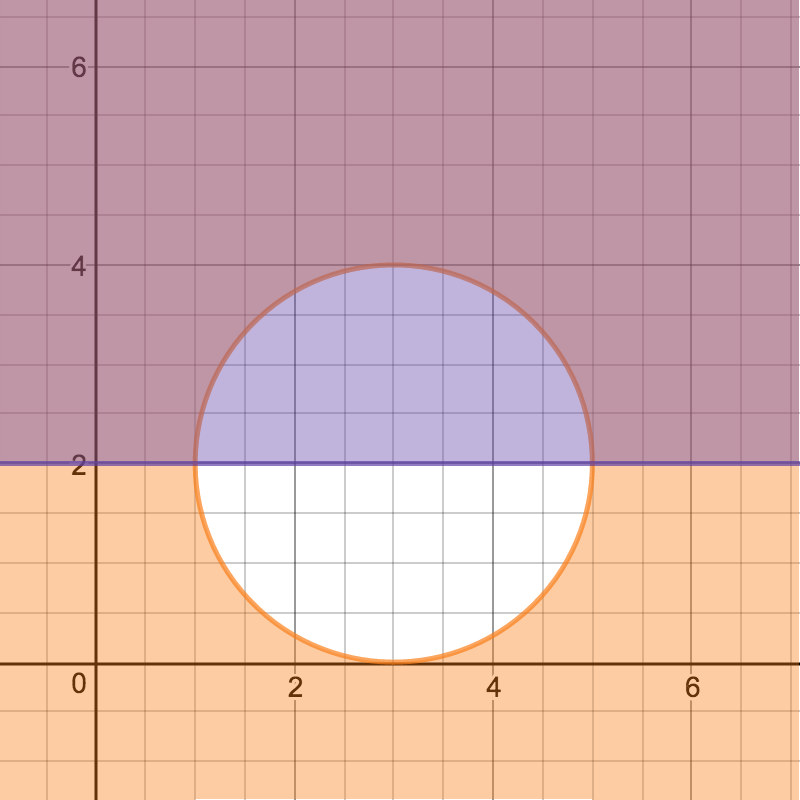
\includegraphics[width=0.8\textwidth]{10022016domain}
		\caption{Dominio della funzione $f(x)$}
	\end{subfigure}
	\caption{La funzione nel suo dominio di definizione}
\end{figure}

b) Le condizioni di Karush-Kuhn-Tucker sono le seguenti:

\begin{theorem}[Condizioni di Karush-Kuhn-Tucker]
	Sia $f$ una funzione, $h_i \text{ con } i \in \{1, \ldots, s\}$ dei vincoli bilateri e $g_j \text{ con } j \in \{1, \ldots, m\}$ dei vincoli monolateri e sia l'insieme $X$ definito come:

	\[
		X  = \{x \in \mathbb{R}^n: g_j(x) \leq 0, h_i(x) = 0 \quad \forall i, j \} \quad \text{e} \quad f, g_j, h_i \in C^1(X) \quad \forall i,j
	\]

	Se $x^*$ è un punto regolare in $X$ e un punto di minimo locale per $f \in X$, allora esistono $s$ moltiplicatori $\lambda_i \in \mathbb{R}$ e $m$ $\mu_j \geq 0$ tali che:

	\begin{align*}
		\nabla f(x^*) + \sum_{i=1}^s \lambda_i \nabla h_i(x^*) + \sum_{j=1}^m \mu_j \nabla g_j(x^*) & = 0 \\
		\mu_j g_j(x^*)                                                                              & = 0
	\end{align*}
\end{theorem}

c) Calcolo dei punti candidati.

\paragraph*{Calcolo dei punti non regolari}
I punti regolari sono quei punti nei quali i gradienti dei vincoli attivi sono fra loro linearmente indipendenti. Punti interni alle regioni di ammissibilità sono tutti regolari. Vanno investigati i punti che annullano il gradiente.

Calcolo quindi i gradienti dei due vincoli, $\nabla g_1(x)$ e $\nabla g_2(x)$:

\[
	\nabla g_1(x) = \begin{bmatrix}
		2x_1 -6 \\
		2x_2 -4
	\end{bmatrix}
	\qquad
	\nabla g_2(x) = \begin{bmatrix}
		0 \\
		1
	\end{bmatrix}
\]

Il primo gradiente si annulla per $P = (x_1 = 3, x_2 = 2)$, che è posto dove si attiva il vincolo $g_2$ ma non $g_1$ ed il secondo gradiente non si annulla mai (menchemeno in $P$) per cui $P$ è considerato regolare.

Identifichiamo ora i punti di intersezione dei vincoli:

\[
	\begin{cases}
		x^2_1+x^2_2-6x_1-4x_2+9  =  0 \\
		x_2-2 = 0
	\end{cases}
	\Rightarrow
	\begin{cases}
		x^2_1+4-6x_1-8+9  =  0 \\
		x_2 = 2
	\end{cases}
	\Rightarrow
	\begin{cases}
		x^2_1-6x_1+5  =  0 \\
		x_2 = 2
	\end{cases}
	\Rightarrow
	\begin{cases}
		x_1 = 3 \pm \sqrt{9 - 5} = 3 \pm 2 \\
		x_2 = 2
	\end{cases}
\]

I punti identificati quindi sono $A = (1, 2)$ e $B = (5, 2)$.

Verifichiamo che i gradienti siano linearmente indipendenti tramite il metodo della matrice: se per uno di essi fossero dipendenti (cioè la matrice ha determinante 0) allora $A$ non sarebbe regolare e le condizioni KKT perderebbero di validità.

\[
	\det M_g(A) = \det\begin{bmatrix}\nabla g_1(A) & \nabla g_2(A)\end{bmatrix}= \det\begin{bmatrix}
		-4 & 0 \\
		0  & 1
	\end{bmatrix}
	= -4 \neq 0
\]

\[
	\det M_g(B) = \det\begin{bmatrix}\nabla g_1(B) & \nabla g_2(B)\end{bmatrix}= \det\begin{bmatrix}
		4 & 0 \\
		0 & 1
	\end{bmatrix}
	= 4
\]


I gradienti sono linearmente indipendenti sia in $A$ che in $B$, che essendo regolari non sono punti candidati.

\paragraph*{Calcolo della lagrangiana generalizzata}
La formula della lagrangiana generalizzata (figura \ref{lagrangiana_generalizzata}) assomiglia molto alle condizioni KKT ma si applica sulle primitive (non i gradienti).

\begin{figure}
	\[
		l(x) = f(x) + \sum_{i=1}^s \lambda_i h_i(x) + \sum_{j=1}^m \mu_j g_j(x)
	\]
	\caption{Formula della lagrangiana generalizzata}
	\label{lagrangiana_generalizzata}
\end{figure}

\begin{align*}
	l(x) & = f(x) + \mu_1 g_1(x) + \mu_2 g_2(x)                               \\
	     & = x^2_2+x_1-4x_2 + \mu_1 (x^2_1+x^2_2-6x_1-4x_2+9) + \mu_2 (x_2-2)
\end{align*}

\paragraph*{Costruisco il sistema delle condizioni KKT}

\[
	\begin{cases}
		\nabla l(x) = \begin{bmatrix}
			1 + \mu_1(2x_1 - 6)                   \\
			2x_2 -4 + \mu_1(2x_2 - 4) + \mu_2 x_2 \\
		\end{bmatrix}
		= \bm{0}                            \\
		\mu_1 (x^2_1+x^2_2-6x_1-4x_2+9) = 0 \\
		\mu_2 (x_2-2) = 0                   \\
		x^2_1+x^2_2-6x_1-4x_2+9 \leq 0      \\
		x_2-2 \leq 0                        \\
		\mu_1 \geq 0                        \\
		\mu_2 \geq 0
	\end{cases}
	\Rightarrow
	\begin{cases}
		\mu_1(2x_1 - 6) = -1                      \\
		2x_2 -4 + \mu_1(2x_2 - 4) + \mu_2 x_2 = 0 \\
		\mu_2 (x_2-2) = 0                         \\
		x^2_1+x^2_2-6x_1-4x_2+9 = 0               \\
		x_2 \leq 2                                \\
		\mu_1 > 0                                 \\
		\mu_2 \geq 0
	\end{cases}
\]

Notiamo che $\mu_1$ deve essere strettamente maggiore di 0, altrimenti la prima equazione $\mu_1(2x_1 - 6) = -1$ non sarebbe rispettata. Se $\mu_1 > 0$, allora $g_1 = 0$.

Impostiamo un albero di ricerca dicotomico per risolvere il sistema, dividendo tra:

\[
	\mu_j = 0 \land g_j \leq 0 \quad \lor \quad \mu_j > 0 \land g_j = 0 \qquad \forall j \in \{1, \ldots, m\}
\]

Iniziamo scegliendo il vincolo più semplice, nel nostro caso $g_2$:

\paragraph*{Caso in cui $\mu_2 = 0 \land g_2 \leq 0$:}
\[
	\begin{cases}
		\mu_1(2x_1 - 6) = -1          \\
		2x_2 -4 + \mu_1(2x_2 - 4) = 0 \\
		x^2_1+x^2_2-6x_1-4x_2+9 = 0   \\
		x_2 \leq 2                    \\
		\mu_1 > 0
	\end{cases}
	\Rightarrow
	\begin{cases}
		\mu_1(2x_1 - 6) = -1           \\
		\textcolor{red!90}{\mu_1 = -1} \\
		x^2_1+x^2_2-6x_1-4x_2+9 = 0    \\
		x_2 \leq 2                     \\
		\textcolor{red!90}{\mu_1 > 0}
	\end{cases}
\]

Ponendo $\mu_2 = 0 \land g_2 \leq 0$ si ottiene che $\mu_1 = -1 \land \mu_1 > 0$, per cui il sistema è impossibile. Se restringiamo il caso in analisi a $\mu_2 = 0 \land g_2 = 0$ è possibile rispettare il vincolo $\mu_1 > 0$ proseguendo così:

\[
	\begin{cases}
		\mu_1(2x_1 - 6) = -1        \\
		0 = 0                       \\
		x^2_1+x^2_2-6x_1-4x_2+9 = 0 \\
		x_2 = 2                     \\
		\mu_1 > 0
	\end{cases}
	\Rightarrow
	\begin{cases}
		\mu_1(2x_1 - 6) = -1 \\
		x^2_1+4-6x_1-8+9 = 0 \\
		x_2 = 2              \\
		\mu_1 > 0
	\end{cases}
	\Rightarrow
	\begin{cases}
		\mu_1(2x_1 - 6) = -1 \\
		x^2_1-6x_1 = -5      \\
		x_2 = 2              \\
		\mu_1 > 0
	\end{cases}
	\Rightarrow
	\begin{cases}
		\mu_1 = -\frac{1}{2x_1 - 6}               \\
		x_1 = 3 \pm \sqrt{9 + 5} = 3 \pm \sqrt{4} \\
		x_2 = 2                                   \\
		\mu_1 > 0
	\end{cases}
\]

Solamente $x_1 = 1$ è accettabile poiché $\mu_1 > 0$:

\[
	\begin{cases}
		\mu_1 = -\frac{1}{2 - 6} =  \frac{1}{4} \\
		x_1 = 1                                 \\
		x_2 = 2
	\end{cases}
\]

Ne otteniamo quindi il punto candidato coincidente con $A = (1, 2)$, con $\bm{\mu} = \begin{bmatrix}
		\frac{1}{4} \\
		0
	\end{bmatrix}$.

\paragraph*{Caso in cui $\mu_2 > 0 \land g_2 = 0$:}
\[
	\begin{cases}
		\mu_1(2x_1 - 6)  = -1                     \\
		2x_2 -4 + \mu_1(2x_2 - 4) + \mu_2 x_2 = 0 \\
		x^2_1+x^2_2-6x_1-4x_2+9 = 0               \\
		x_2 = 2                                   \\
		\mu_1 > 0                                 \\
		\mu_2 > 0
	\end{cases}
	\Rightarrow
	\begin{cases}
		\mu_1(2x_1 - 6)  = -1            \\
		4 -4 + \mu_1(4 - 4) + 2\mu_2 = 0 \\
		x^2_1+4-6x_1-8+9 = 0             \\
		x_2 = 2                          \\
		\mu_1 > 0                        \\
		\mu_2 > 0
	\end{cases}
	\Rightarrow
	\begin{cases}
		\mu_1(2x_1 - 6)  = -1        \\
		\textcolor{red!90}{\mu_2 =0} \\
		x^2_1+4-6x_1-8+9 = 0         \\
		x_2 = 2                      \\
		\mu_1 > 0                    \\
		\textcolor{red!90}{\mu_2 > 0}
	\end{cases}
\]

Ponendo $\mu_2 > 0 \land g_2 = 0$ si ottiene che $\mu_2 = 0 \land \mu_2 > 0$, per cui il sistema è impossibile. Ne segue che il caso in analisi è impossibile.

\paragraph*{Calcolo del valore dei punti candidati}
Sostituisco i punti candidati nella funzione da minimizzare ed ottengo:

\[
	\begin{cases}
		f(A) = f(1,2) =  4 + 1 - 8 = -3 \\
	\end{cases}
\]

Il punto di ottimo locale (minimo) risulta essere $A = (1, 2)$.

\end{document}